\documentclass[xcolor=x11names,compress,8pt]{beamer}
\usepackage{graphicx}
\usepackage{amsmath}
\usepackage{hyperref}
\hypersetup{
    colorlinks=true,
    linkcolor=GopherMaroon, % Internal navigation links
    filecolor=GopherMaroon,
    urlcolor=blue,          % External hyperlinks (URLs)
    citecolor=GopherMaroon,
}

%% UMN Template Setup
\xdefinecolor{GopherMaroon}{HTML}{7A0019}
\xdefinecolor{GopherGold}{HTML}{FFCC33}
\xdefinecolor{GopherLightGold}{HTML}{FFDE7A}
\xdefinecolor{GopherDarkMaroon}{HTML}{5B0013}

\useoutertheme[subsection=false,shadow]{miniframes}
\useinnertheme{default}
\usefonttheme{serif}
\usepackage{palatino}

\setbeamerfont{title like}{shape=\scshape}
\setbeamerfont{frametitle}{shape=\scshape}

\setbeamercolor*{lower separation line head}{bg=GopherMaroon} 
\setbeamercolor*{normal text}{fg=black,bg=white} 
\setbeamercolor*{alerted text}{fg=red} 
\setbeamercolor*{example text}{fg=black} 
\setbeamercolor*{structure}{fg=black} 
 
\setbeamercolor*{palette tertiary}{fg=GopherDarkMaroon,bg=GopherLightGold} 
\setbeamercolor*{palette quaternary}{fg=GopherDarkMaroon,bg=GopherLightGold}

\def\Circlearrowleft{\ensuremath{%
  \rotatebox[origin=c]{180}{$\circlearrowleft$}}}
\def\Circlearrowright{\ensuremath{%
  \rotatebox[origin=c]{180}{$\circlearrowright$}}}
\def\CircleArrowleft{\ensuremath{%
  \reflectbox{\rotatebox[origin=c]{180}{$\circlearrowleft$}}}}
\def\CircleArrowright{\ensuremath{%
  \reflectbox{\rotatebox[origin=c]{180}{$\circlearrowright$}}}}

\usepackage[T1]{fontenc}
\usepackage{concrete}
\usepackage{amsmath,amsthm,amssymb}
\usepackage{multicol}
\usepackage{caption}
\usepackage{subcaption}
\usepackage{standalone}
\usepackage{tkz-graph}
\usepackage{tikz,mathabx}
\usetikzlibrary{positioning}
\usetikzlibrary{shapes}
\usepackage{amsfonts}
\usepackage{mathtools}
\usepackage[normalem]{ulem}
\usepackage{adjustbox, centernot}
\usepackage{wrapfig,graphicx}
\theoremstyle{plain}
  \newtheorem{conjecture}{Conjecture}
  \newtheorem{observation}{Observation}
\renewcommand{\rmdefault}{pplx}
\setbeamertemplate{navigation symbols}{}

\newcommand{\GG}{\ensuremath{\mathcal{G}}}
\newcommand{\ZZ}{\ensuremath{\mathbb{Z}}}
\DeclarePairedDelimiter\ceil{\lceil}{\rceil} % Command for ceiling function : \ceil{x}
\DeclarePairedDelimiter\floor{\lfloor}{\rfloor} % Command for floor function: \floor{x}
\newcommand{\Mod}[1]{\ (\mathrm{mod}\ #1)}
\title{G-decompositions and G-designs for Forests with Seven Edges}
\author{Danny Banegas, Professor Bryan Freyberg}
\institute{University of Minnesota: Duluth}
\date{\today}

\begin{document}

% Title Slide
{
\setbeamertemplate{footline}{}
\begin{frame}
    \centering
    \includegraphics[width=0.3\textwidth]{logoumn} \\[1em]
    \titlepage
\end{frame}
}

% Outline Slide
\begin{frame}{Outline}
\tableofcontents
\end{frame}

% Section: Forest Graphs
\section{Forest Graphs}

% Frame: Forest Graphs
\begin{frame}{Forest Graphs}
    \begin{itemize}
    \pause
        \item A \textbf{forest} is a disjoint union of trees.
        \pause
        \item It consists of multiple components, each being a tree.
    \end{itemize}
    \pause
    \begin{figure}
        \centering
        \begin{tikzpicture}[scale=1.5]
            % Tree 1
            \node[circle, draw] (a1) at (0,0) {};
            \node[circle, draw] (b1) at (-0.5,-1) {};
            \node[circle, draw] (c1) at (0.5,-1) {};
            \draw (a1) -- (b1);
            \draw (a1) -- (c1);
            
            % Tree 2
            \node[circle, draw] (a2) at (2,0) {};
            \node[circle, draw] (b2) at (1.5,-1) {};
            \node[circle, draw] (c2) at (2.5,-1) {};
            \node[circle, draw] (d2) at (2,-2) {};
            \draw (a2) -- (b2);
            \draw (a2) -- (c2);
            \draw (c2) -- (d2);
        \end{tikzpicture}
        \caption{A Forest graph composed of trees with $3$ and $4$ vertices, respectively }
    \end{figure}
\end{frame}


\section{Decompositions and Designs}
%frame 1
\begin{frame}{Decompositions and Designs}
    \pause
    \begin{itemize}
        \item We call a set $\GG = \{G_{0}, G_{1}, \hdots, G_{m}\}$ of pairwise edge-disjoint subgraphs of a graph $K$ a decomposition of $K$ if the union of all of its members equals $K$.
        \pause
        \item If $\GG$ is a decomposition of $K$ and all of it's members are isomorphic to some graph $G$, then we call $\GG$ a $G-$decomposition of $K$ and say that $K$ allows a $G-$decomposition or \textbf{$(K,G)-$design}.
        \pause
        \item If $K\cong K_{n}$ then we call $\GG$ a \textbf{$G-$design} of order $n$.
        \pause
    \end{itemize}
    \begin{figure}
        \begin{center}
            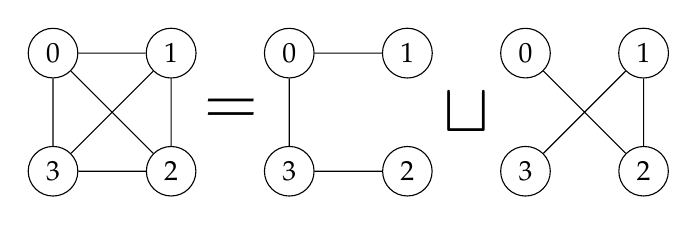
\begin{tikzpicture}[scale=1.5]
                % First graph
                \node (0) at (0, 0) [circle, draw] {0};
                \node (1) at (1, 0) [circle, draw] {1};
                \node (2) at (1, -1) [circle, draw] {2};
                \node (3) at (0, -1) [circle, draw] {3};
    
                \draw (2) -- (3) -- (0) -- (1);
                \draw (0) -- (2) -- (1) -- (3);
                \pause
                % "=" symbol
                \node at (1.5, -0.5) {\Huge $=$};
    
                % Second graph
                \begin{scope}[xshift=2cm]
                    \node (0) at (0, 0) [circle, draw] {0};
                    \node (1) at (1, 0) [circle, draw] {1};
                    \node (2) at (1, -1) [circle, draw] {2};
                    \node (3) at (0, -1) [circle, draw] {3};
    
                    \draw (1) -- (0) -- (3) -- (2);
                \end{scope}
                \pause
                % "\cup" symbol
                \node at (3.5, -0.5) {\Huge $\sqcup$};
                
                \begin{scope}[xshift=4cm]
                    \node (0) at (0, 0) [circle, draw] {0};
                    \node (1) at (1, 0) [circle, draw] {1};
                    \node (2) at (1, -1) [circle, draw] {2};
                    \node (3) at (0, -1) [circle, draw] {3};
                    
                    \draw (0) -- (2) -- (1) -- (3);
                \end{scope}
            \end{tikzpicture}
        \end{center}
        \caption{A $P_{3}-$Design of order $4$}
    \end{figure}
\end{frame}

%necessary conditions
\begin{frame}{Necessary condition}
\begin{itemize}
\item Let $G$ be a graph on $m$ edges. Then there exists a $(K,G)-$design only if $m$ divides $|E(K)|$.
\pause
\item If $K\cong K_{n}$, then there exists a $(K,G)-$design only if $m$ divides $\binom{n}{2}=\frac{n(n-1)}{2}$.
\pause
\item Equivalently, there exists a $G-$design of order $n$ only if $n$ is idempotent modulo $2m$.  This is easy to show.
\pause
\end{itemize}

\begin{proof}
    Let $m,n\in \mathbb{N}$. Suppose $m \mid \binom{n}{2}$. Then $\frac{n(n-1)}{2} = mq$ for some $q \in \mathbb{N}$. So then $\frac{n(n-1)}{2m} = q$, and $n(n-1) \equiv 0 \pmod{2m}$. Therefore $n \equiv n^2 \pmod{2m}$, and so $n$ is idempotent modulo $2m$. Suppose $n$ is idempotent modulo $2m$, then $n^{2}>n$ and therefore $n^{2}-n=n(n-1)=2mp$ for some $p\in \mathbb{N}$. So then $\frac{n(n-1)}{2}=\binom{n}{2}=mp$ and $m$ divides $\binom{n}{2}._{\;\;\qedsymbol}$ 
    \end{proof}
\end{frame}
% cyclic G-decompositions and G-designs
\begin{frame}{Cyclic Designs}
    \pause
    \begin{itemize}
    \item Let $V(K_n)=\mathbb{Z}_n$
    \pause
    \item A $G$-design is \emph{cyclic} if the permutation $v\mapsto v+1$ on $V(K_n)$ is an automorphism of the design.
    \pause
    \item We call this act of applying permutations to a labeling \emph{clicking}.
    \end{itemize}
    \end{frame}

%nodes placed---------------------------------------------------------------------
\begin{frame}{An example of a cyclic design}
    \textbf{Cyclic $P_3$-design of order 5}\\

    \begin{figure}
        \centering
        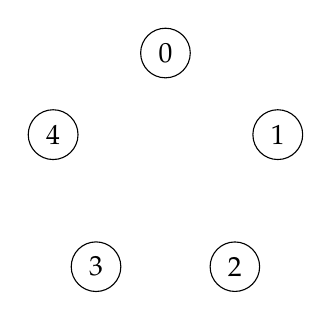
\begin{tikzpicture}[scale=1.5]
            % Define the vertices
            \node[circle, draw=black, fill=white, text=black] (0) at (90:1) {0};
            \node[circle, draw=black, fill=white, text=black] (1) at (18:1) {1};
            \node[circle, draw=black, fill=white, text=black] (2) at (306:1) {2};
            \node[circle, draw=black, fill=white, text=black] (3) at (234:1) {3};
            \node[circle, draw=black, fill=white, text=black] (4) at (162:1) {4};
            
        \end{tikzpicture}
    \end{figure}
\end{frame}
%click black----------------------------------------------------------------------
\begin{frame}{An example of a cyclic design}
    \textbf{Cyclic $P_3$-design of order 5}\\
    \color{black} $\{1,0,3\}$ \newline
    
    \begin{figure}
        \centering
        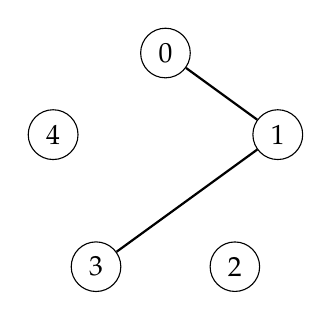
\begin{tikzpicture}[scale=1.5]
            % Define the vertices
            \node[circle, draw=black, fill=white, text=black] (0) at (90:1) {0};
            \node[circle, draw=black, fill=white, text=black] (1) at (18:1) {1};
            \node[circle, draw=black, fill=white, text=black] (2) at (306:1) {2};
            \node[circle, draw=black, fill=white, text=black] (3) at (234:1) {3};
            \node[circle, draw=black, fill=white, text=black] (4) at (162:1) {4};
            
            % Draw the edges of the P_3 subgraphs
            \draw[black, thick] (0) -- (1) -- (3);
        \end{tikzpicture}
    \end{figure}
\end{frame}
%click red------------------------------------------------------------------------
\begin{frame}{An example of a cyclic design}
    \textbf{Cyclic $P_3$-design of order 5}\\
    \color{black} $\{1,0,3\}$ \newline
    \color{red} $\{2,1,4\}$ \newline

    \begin{figure}
        \centering
        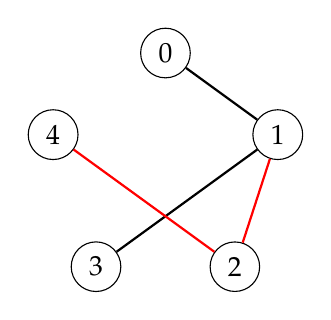
\begin{tikzpicture}[scale=1.5]
            % Define the vertices
            \node[circle, draw=black, fill=white, text=black] (0) at (90:1) {0};
            \node[circle, draw=black, fill=white, text=black] (1) at (18:1) {1};
            \node[circle, draw=black, fill=white, text=black] (2) at (306:1) {2};
            \node[circle, draw=black, fill=white, text=black] (3) at (234:1) {3};
            \node[circle, draw=black, fill=white, text=black] (4) at (162:1) {4};
            
            % Draw the edges of the P_3 subgraphs
            \draw[black, thick] (0) -- (1) -- (3);
            \draw[red, thick] (1) -- (2) -- (4);
        \end{tikzpicture}
    \end{figure}
\end{frame}
%click blue-----------------------------------------------------------------------
\begin{frame}{An example of a cyclic design}
    \textbf{Cyclic $P_3$-design of order 5}\\
    \color{black} $\{1,0,3\}$ \newline
    \color{red} $\{2,1,4\}$ \newline
    \color{blue} $\{3,2,0\}$ \newline

    \begin{figure}
        \centering
        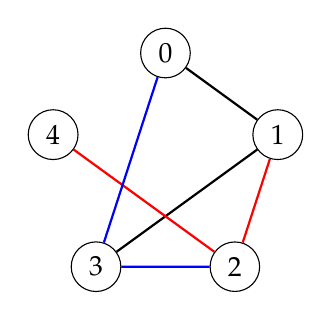
\begin{tikzpicture}[scale=1.5]
            % Define the vertices
            \node[circle, draw=black, fill=white, text=black] (0) at (90:1) {0};
            \node[circle, draw=black, fill=white, text=black] (1) at (18:1) {1};
            \node[circle, draw=black, fill=white, text=black] (2) at (306:1) {2};
            \node[circle, draw=black, fill=white, text=black] (3) at (234:1) {3};
            \node[circle, draw=black, fill=white, text=black] (4) at (162:1) {4};
            
            % Draw the edges of the P_3 subgraphs
            \draw[black, thick] (0) -- (1) -- (3);
            \draw[red, thick] (1) -- (2) -- (4);
            \draw[blue, thick] (2) -- (3) -- (0);
        \end{tikzpicture}
    \end{figure}
\end{frame}
%click green--------------------------------------------------------------------
\begin{frame}{An example of a cyclic design}
    \textbf{Cyclic $P_3$-design of order 5}\\
    \color{black} $\{1,0,3\}$ \newline
    \color{red} $\{2,1,4\}$ \newline
    \color{blue} $\{3,2,0\}$ \newline
    \color{green} $\{4,3,1\}$ \newline

    \begin{figure}
        \centering
        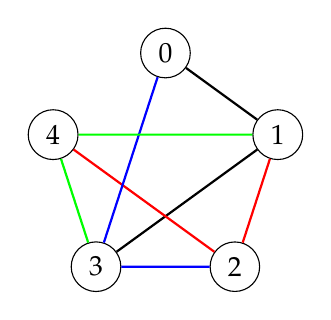
\begin{tikzpicture}[scale=1.5]
            % Define the vertices
            \node[circle, draw=black, fill=white, text=black] (0) at (90:1) {0};
            \node[circle, draw=black, fill=white, text=black] (1) at (18:1) {1};
            \node[circle, draw=black, fill=white, text=black] (2) at (306:1) {2};
            \node[circle, draw=black, fill=white, text=black] (3) at (234:1) {3};
            \node[circle, draw=black, fill=white, text=black] (4) at (162:1) {4};
            
            % Draw the edges of the P_3 subgraphs
            \draw[black, thick] (0) -- (1) -- (3);
            \draw[red, thick] (1) -- (2) -- (4);
            \draw[blue, thick] (2) -- (3) -- (0);
            \draw[green, thick] (3) -- (4) -- (1);
        \end{tikzpicture}
    \end{figure}
\end{frame}
%click magenta--------------------------------------------------------------------
\begin{frame}{An example of a cyclic design}
    \textbf{Cyclic $P_3$-design of order 5}\\
    \color{black} $\{1,0,3\}$ \newline
    \color{red} $\{2,1,4\}$ \newline
    \color{blue} $\{3,2,0\}$ \newline
    \color{green} $\{4,3,1\}$ \newline
    \color{magenta} $\{0,4,2\}$

    \begin{figure}
        \centering
        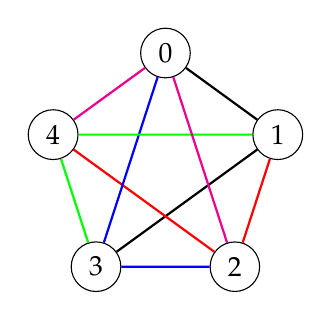
\begin{tikzpicture}[scale=1.5]
            % Define the vertices
            \node[circle, draw=black, fill=white, text=black] (0) at (90:1) {0};
            \node[circle, draw=black, fill=white, text=black] (1) at (18:1) {1};
            \node[circle, draw=black, fill=white, text=black] (2) at (306:1) {2};
            \node[circle, draw=black, fill=white, text=black] (3) at (234:1) {3};
            \node[circle, draw=black, fill=white, text=black] (4) at (162:1) {4};
            
            % Draw the edges of the P_3 subgraphs
            \draw[black, thick] (0) -- (1) -- (3);
            \draw[red, thick] (1) -- (2) -- (4);
            \draw[blue, thick] (2) -- (3) -- (0);
            \draw[green, thick] (3) -- (4) -- (1);
            \draw[magenta, thick] (4) -- (0) -- (2);
        \end{tikzpicture}
        \caption{Cyclic $P_3$-design of order 5}
    \end{figure}
\end{frame}

\section{Edge Length and Decompositions}
\begin{frame}{Edge length}
\begin{itemize}
\item Let $V(K_n)=\{0,1,\hdots,n-1\}$ 
\pause
\item The \emph{length} of edge $uv \in E(K_n)$ is $\min(|u-v|,n-|u-v|)$ and will later be denoted $\ell(uv)$.
\pause
\item If the length of $uv$ is $n-|u-v|\text{ or equivalently, if } |u-v|>\floor{\frac{n}{2}},$ then we call $xy$ a \emph{wrap-around} edge
\end{itemize}
\end{frame}

\begin{frame}{Edge Length and Decompositions}
    \begin{itemize}
        \item Edge length is preserved by the permutation $v\mapsto v+1$ on $V(K_n)$
        \pause
        \item Also, when $n$ is odd, edge length partitions $E(K_n)$ into $\frac{n-1}{2}$ (the number of lengths) sets of size $n$ (the number of edges of each length) 
        \pause
    \end{itemize}
    \begin{center}
        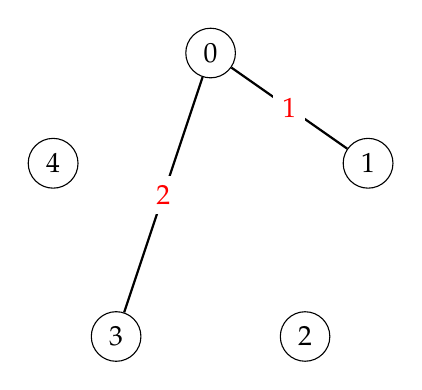
\begin{tikzpicture}[scale=0.2]
       
        
     \node[circle, draw=black, fill=white, text=black](0) at (0,10) {0};
     \node[circle, draw=black, fill=white, text=black](1) at (10,3) {1};
     \node[circle, draw=black, fill=white, text=black](2) at (6,-8) {2};
     \node[circle, draw=black, fill=white, text=black](3) at (-6,-8) {3};
     \node[circle, draw=black, fill=white, text=black](4) at (-10,3) {4};
    \tikzset{EdgeStyle/.style={}} 
        \draw[black, thick] (0) -- (1) node[midway, text=red, fill=white] {1};
        \draw[black, thick] (0) -- (3) node[midway, text=red, fill=white] {2};
        
        \end{tikzpicture}
    \end{center}
        
    \end{frame}
    %-----------click-----
    \begin{frame}
    \frametitle{Edge Length and Decompositions}
    \begin{itemize}
        \item Edge length is preserved by the permutation $v\mapsto v+1$ on $V(K_n)$
        \item Also, when $n$ is odd, edge length partitions $E(K_n)$ into $\frac{n-1}{2}$ (the number of lengths) sets of size $n$ (the number of edges of each length) 
    \end{itemize}
    \begin{center}
        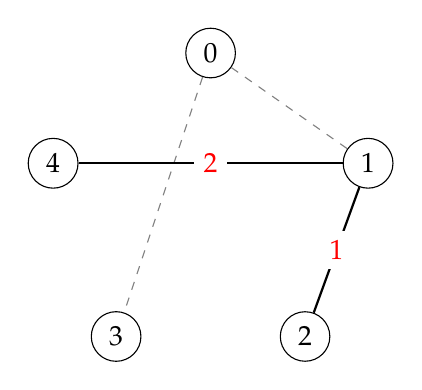
\begin{tikzpicture}[scale=0.2]
       
        
     \node[circle, draw=black, fill=white, text=black](0) at (0,10) {0};
     \node[circle, draw=black, fill=white, text=black](1) at (10,3) {1};
     \node[circle, draw=black, fill=white, text=black](2) at (6,-8) {2};
     \node[circle, draw=black, fill=white, text=black](3) at (-6,-8) {3};
     \node[circle, draw=black, fill=white, text=black](4) at (-10,3) {4};
     
            \draw[gray, dashed](0)--(1);
            \draw[gray, dashed](0)--(3);
            \tikzset{EdgeStyle/.style={}} 
            \draw[black, thick] (4) -- (1) node[midway, text=red, fill=white] {2};
            \draw[black, thick] (1) -- (2) node[midway, text=red, fill=white] {1};
          
        \end{tikzpicture}
    \end{center}
        
    \end{frame}
    %-click---------------
    \begin{frame}
    \frametitle{Edge Length and Decompositions}
    \begin{itemize}
        \item Edge length is preserved by the permutation $v\mapsto v+1$ on $V(K_n)$
        \item Also, when $n$ is odd, edge length partitions $E(K_n)$ into $\frac{n-1}{2}$ (the number of lengths) sets of size $n$ (the number of edges of each length) 
    \end{itemize}
    \begin{center}
        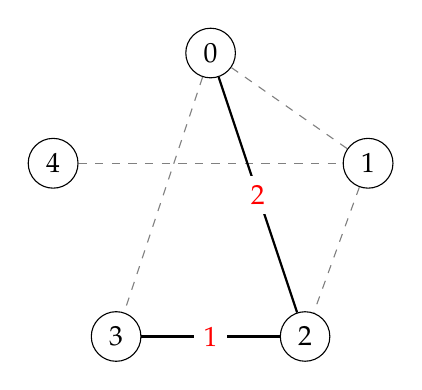
\begin{tikzpicture}[scale=0.2]
       
        
     \node[circle, draw=black, fill=white, text=black](0) at (0,10) {0};
     \node[circle, draw=black, fill=white, text=black](1) at (10,3) {1};
     \node[circle, draw=black, fill=white, text=black](2) at (6,-8) {2};
     \node[circle, draw=black, fill=white, text=black](3) at (-6,-8) {3};
     \node[circle, draw=black, fill=white, text=black](4) at (-10,3) {4};
     
            \draw[gray, dashed](0)--(1);
            \draw[gray, dashed](0)--(3);
     
            \draw[gray, dashed](4)--(1);
            \draw[gray, dashed](1)--(2);
    \tikzset{EdgeStyle/.style={}} 
            \draw[black, thick] (0) -- (2) node[midway, text=red, fill=white] {2};
            \draw[black, thick] (3) -- (2) node[midway, text=red, fill=white] {1};
        \end{tikzpicture}
    \end{center}
        
    \end{frame}
    %---click-----------
    \begin{frame}
    \frametitle{Edge Length and Decompositions}
    \begin{itemize}
        \item Edge length is preserved by the permutation $v\mapsto v+1$ on $V(K_n)$
        \item Also, when $n$ is odd, edge length partitions $E(K_n)$ into $\frac{n-1}{2}$ (the number of lengths) sets of size $n$ (the number of edges of each length) 
    \end{itemize}
    \begin{center}
        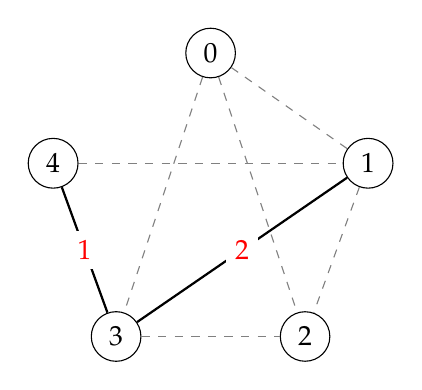
\begin{tikzpicture}[scale=0.2]
       
        
     \node[circle, draw=black, fill=white, text=black](0) at (0,10) {0};
     \node[circle, draw=black, fill=white, text=black](1) at (10,3) {1};
     \node[circle, draw=black, fill=white, text=black](2) at (6,-8) {2};
     \node[circle, draw=black, fill=white, text=black](3) at (-6,-8) {3};
     \node[circle, draw=black, fill=white, text=black](4) at (-10,3) {4};
      
            \draw[gray, dashed](0)--(1);
            \draw[gray, dashed](0)--(3);
             
            \draw[gray, dashed](4)--(1);
            \draw[gray, dashed](1)--(2);
           
            \draw[gray, dashed](0)--(2);
            \draw[gray, dashed](3)--(2);
    \tikzset{EdgeStyle/.style={}}         
        \draw[black, thick] (1) -- (3) node[midway, text=red, fill=white] {2};
        \draw[black, thick] (3) -- (4) node[midway, text=red, fill=white] {1};
          
        \end{tikzpicture}
    \end{center}
        
    \end{frame}
    %----click------
    \begin{frame}
    \frametitle{Edge Length and Decompositions}
    \begin{itemize}
        \item Edge length is preserved by the permutation $v\mapsto v+1$ on $V(K_n)$
        \item Also, when $n$ is odd, edge length partitions $E(K_n)$ into $\frac{n-1}{2}$ (the number of lengths) sets of size $n$ (the number of edges of each length) 
    \end{itemize}
    \begin{center}
        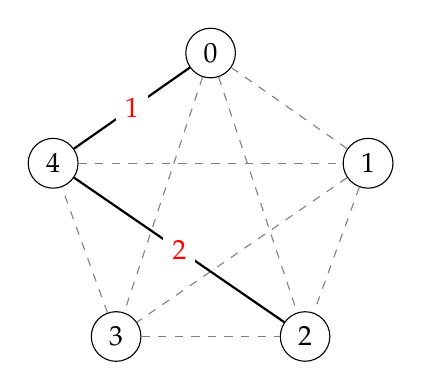
\begin{tikzpicture}[scale=0.2]
       
        
     \node[circle, draw=black, fill=white, text=black](0) at (0,10) {0};
     \node[circle, draw=black, fill=white, text=black](1) at (10,3) {1};
     \node[circle, draw=black, fill=white, text=black](2) at (6,-8) {2};
     \node[circle, draw=black, fill=white, text=black](3) at (-6,-8) {3};
     \node[circle, draw=black, fill=white, text=black](4) at (-10,3) {4};
     
            \draw[gray, dashed](0)--(1);
            \draw[gray, dashed](0)--(3);
     
            \draw[gray, dashed](4)--(1);
            \draw[gray, dashed](1)--(2);
           
            \draw[gray, dashed](0)--(2);
            \draw[gray, dashed](3)--(2);

            \draw[gray, dashed](1)--(3);
            \draw[gray, dashed](3)--(4);

     \tikzset{EdgeStyle/.style={}}    
            \draw[black, thick] (2) -- (4) node[midway, text=red, fill=white] {2};
            \draw[black, thick] (0) -- (4) node[midway, text=red, fill=white] {1};
        \end{tikzpicture}
    \end{center}
        
    \end{frame}
    %----click------
    \begin{frame}{Edge Length and Decompositions}
    \begin{itemize}
        \item Edge length is preserved by the permutation $v\mapsto v+1$ on $V(K_n)$
        \item Also, when $n$ is odd, edge length partitions $E(K_n)$ into $\frac{n-1}{2}$ (the number of lengths) sets of size $n$ (the number of edges of each length) 
    \end{itemize}
    \begin{center}
        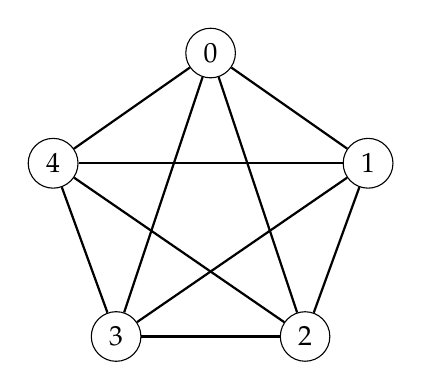
\begin{tikzpicture}[scale=0.2]
    
     \node[circle, draw=black, fill=white, text=black](0) at (0,10) {0};
     \node[circle, draw=black, fill=white, text=black](1) at (10,3) {1};
     \node[circle, draw=black, fill=white, text=black](2) at (6,-8) {2};
     \node[circle, draw=black, fill=white, text=black](3) at (-6,-8) {3};
     \node[circle, draw=black, fill=white, text=black](4) at (-10,3) {4};

            \draw[black, thick](0)--(1);
            \draw[black, thick](0)--(3);

            \draw[black, thick](4)--(1);
            \draw[black, thick](1)--(2);
      
            \draw[black, thick](0)--(2);
            \draw[black, thick](3)--(2);
    
            \draw[black, thick](1)--(3);
            \draw[black, thick](3)--(4);
    
            \draw[black, thick] (2) -- (4);
            \draw[black, thick] (0) -- (4);
        \end{tikzpicture}
    \end{center}
        
    \end{frame}
    % Section: sigma labelings
\section{$\sigma^{+-}$-labelings}
    \begin{frame}{$\sigma^{+-}$-labelings}
        \begin{itemize}
            \item Recall the length of  $uv \in E(K_n)$ is min$(|u-v|,n-|u-v|).$
            \pause
            \item A $\sigma$-labeling is a labeling such that the length of every edge $uv \in E(K_n)$ is $|u-v|.$
            \pause
            \item Freyberg and Tran introduced the following restricted $\sigma$-labeling in 2020.
        \end{itemize}
        \begin{definition}
         Let $G$ be a bipartite graph with $m$ edges and bipartition $V(G)=A\cup B$. A $\sigma^{+-}$-\emph{labeling} of $G$ is a $\sigma$-labeling with:
        \begin{enumerate}
            \item $f(a)<f(b)$ for every edge $ab\in E(G)$ with $a\in A$ and $b \in B$
            \item $f(a)-f(b) \neq m$ for all $a,b \in V(G)$
            \item $f(v) \not \in \{2m-1,2m\}$ for all $v \in V(G)$
        \end{enumerate}   
        \end{definition}    
        
        \end{frame}
        %------------
        \begin{frame}{$\sigma^{+-}$-labelings}
            \begin{theorem} [Freyberg, Tran, 2020] 
        Let $G$ be a graph with $m$ edges and a $\sigma^{+-}$-labeling such that the edge of length $m$ is a pendant edge. Then there exists cyclic $G$-decompositions of $K_{2mt}$ and $K_{2mt+1}$ for every positive integer $t.$
        \end{theorem}
        
        \end{frame}

    \begin{frame}{$7$ edge forest G-decompositions and G-designs}
        \begin{itemize}
            \item Recall that if $G$ has $m$ edges, then there exists a $G$-design of order $n$ only if $n$ is idempotent modulo $2m$.
            \item So $F$ is a forest on $7$ edges, there exists an $F$-design of order $n$ only if $n\equiv 0,1,7,\text{ or }8\Mod{14}$, since those are all the idempotents in $\ZZ_{14}$.
            \item So by Freyberg and Tran, if there exists a $\sigma^{+-}$-labeling of all forests $F$ on $7$ edges, then there exists $F$-G-decompositions and G-designs of order $14t$ and $14t+1$ for all $t>0$ and all forests $F$ on $7$ edges.
        \end{itemize}
    \end{frame}

    \begin{frame}{$7$ edge forest G-decompositions and G-designs}
        \begin{itemize}
        \item The matching on $7$-edges: $\bigsqcup\limits_{i=1}^{7}\,P_{2}$ was solved by De Werra in 1970.

        \item So last summer I found a $\sigma^{+-}$-labeling of all forests on seven edges, up to isomorphism except $\bigsqcup\limits_{i=1}^{7}\,P_{2}$. There are $46$ total excluding the matching.
        \end{itemize}
    \end{frame}

    \begin{frame}{$7$ edge forest G-decompositions and G-designs}
        \begin{figure}
        \begin{center}
            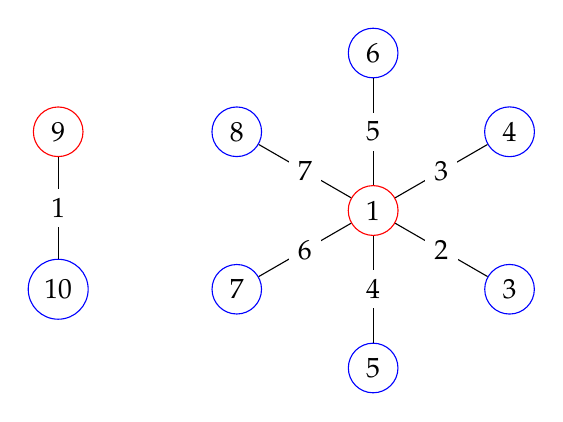
\begin{tikzpicture}[scale=2]
                % Define the vertices in a cycle
                \node (6) at (90:1) [circle, draw=blue] {6};
                \node (4) at (30:1) [circle, draw=blue] {4};
                \node (3) at (330:1) [circle, draw=blue] {3};
                \node (5) at (270:1) [circle, draw=blue] {5};
                \node (7) at (210:1) [circle, draw=blue] {7};
                \node (8) at (150:1) [circle, draw=blue] {8};
                
                % Define the center vertex
                \node (1) at (0,0) [circle, draw=red] {1};
                
                % Define the lone 2-path
                \node (9) at (-2, 0.5) [circle, draw=red] {9};
                \node (10) at (-2, -0.5) [circle, draw=blue] {10};
                
                % Draw the edges in a star
                \draw (1) -- (6) node[midway, text=black, fill=white] {5};
                \draw (1) -- (4) node[midway, text=black, fill=white] {3};
                \draw (1) -- (3) node[midway, text=black, fill=white] {2};
                \draw (1) -- (5) node[midway, text=black, fill=white] {4};
                \draw (1) -- (7) node[midway, text=black, fill=white] {6};
                \draw (1) -- (8) node[midway, text=black, fill=white] {7};
                
                % Draw the lone 2-path
                \draw (9) -- (10)node[midway, text=black, fill=white] {1};
            \end{tikzpicture}
        \end{center}
        \caption{A $\sigma^{+-}$-labeling of $K_{1,7}\sqcup P_{2}$}
    \end{figure}
    \end{frame}
    \begin{frame}{$\sigma^{+-}$-labelings of seven edge forests}
        \textbf{How do these work?}\newline
        \pause
        \begin{itemize}
            \item $\sigma^{+-}$-labelings give these decompositions because there are only lengths $\{1,\hdots,7\}$ in $K_{14}$ and so for for $K_{14t}$ we can simply 'stretch' the \textcolor{blue}{B} partite set on our $\sigma^{+-}$-labeling via $\textcolor{blue}{b}\mapsto \textcolor{blue}{b}+7i$ for each $1\leq i\leq t$ and then \textit{develop} them by $1$; permute all vertices in the labeling via $v\mapsto v+1$,  to generate the new lengths (since they come 7 at a time) and obtain a $G$-design of order $14t$. 
            \pause
            \item This idea also gives G-designs of order $14t+1$ where the new node is labeled $\infty$, and the lengths are still $\{0,\hdots,7\}$ since $\floor{\frac{15}{2}}=7$ plus a new length $\infty$ for each edge incident to the node $\infty$.
            \pause
            \item 

        \end{itemize}

    \end{frame}
    \section{$n\equiv 7\text{ or }8\Mod{14}$}
    \begin{frame}{Non-Cyclic designs: $n\equiv 7\text{ or }8\Mod{14}$}
        \textbf{What about the cases where $n\equiv 7\text{ or }8\Mod{14}$?}
        \begin{itemize}
            \pause
            
            \item Lets just look at the starting case we want for $n\equiv 7\Mod{14}$: $K_{14t+7}$ where $t>0$ or $K_{n}$ where $n\equiv 7\Mod{14}.$ This is $K_{21}$.
            
            \pause

            \item $\floor{\frac{21}{2}}=10$, so we have lengths $\{1,\hdots, 10\}$. This means we can't use the same labeling idea as before to develop a single labeling by $1$, because $7$-edge forest can only fit $7$ distinct lengths$\hdots$
                        
            \pause
            
            \item Well, what if we can collect edges of some lengths $\{a,b,c\}$ from $\{1,\hdots, 10\}$ in some other way for each? Then we can simply take some variation of our $\sigma^{+-}$-labelings accounting for lengths $\{1,\hdots,10\}\setminus \{a,b,c\}$ and develop them by $1$ to get the remaining lengths.
            
            \pause

            \item In the case of $n\equiv 8\Mod{14}$, we look at $\{a,b,c,\infty\}$. If we can successfully do this, we can once again just 'stretch' the \textcolor{blue}{B} partite set of some variation of our $\sigma^{+-}$-labelings to scale up (since new lengths still come 7 at a time).

        \end{itemize}

    \end{frame}

    \begin{frame}{(1-2-3)-labelings and 1-rotational (1-2-3)-labelings}
        We present the following labeling, which allows us to develop $3$ labelings of each forest $G$ by $7$ to collect all edges of lengths in $\{1,2,3\}$ in copies of $G$:
        \begin{definition}\label{def:123}
            Let $G$ be a graph with $7$ edges. A (1-2-3)-\emph{labeling} of $3G$ is an assignment $f$ of the integers $\{0,\dots,20\}$ to the vertices of $3G$ such that:
            \begin{enumerate}
                \item $f(u) \neq f(v)$ whenever $u$ and $v$ belong to the same component
                %\item there are exactly $7$ edges of length $i$ for each $i \in \{1,2,3\}$, and
               % \item if two edges $u_1v_1$ and $u_2v_2$ are of length $i$ and $u_1 \equiv v_1 \pmod7$, then $u_2 \not \equiv v_2 \pmod7.$
              %  \item when $f$ is reduced modulo $7$, there is exactly one edge of length $j$, for $j \in \{1,2,3\}$, of the form $\{i,i+j\}$ for $i \in \{0,\dots,6\}.$
                \item $$\bigcup_{uv\in E(3G)} \{(f(u)\; \textbf{mod } 7,f(v)\; \textbf{mod } 7)\}= \bigcup_{i=0}^{6} \bigcup_{j=1}^{3} \{(i,i+j \; \textbf{mod } 7)\}$$
            \end{enumerate}
        \end{definition}

    \end{frame}

    \begin{frame}{(1-2-3)-labelings and 1-rotational (1-2-3)-labelings}
        Similarly, we present the 1-rotational version of this labeling which allows us to develop $4$ labelings of each forest $G$ by $7$ to collect all edges of lengths in $\{1,2,3,\infty\}$ in copies of $G$
        \begin{definition}\label{def:123_1-rot}
            Let $G$ be a graph with $7$ edges. A \emph{1-rotational $(1$-$2$-$3)$-labeling} of $4G$ is an assignment $f$ of $\{0,\dots,20\} \cup \infty$ to the vertices of $4G$ such that
            \begin{enumerate}
                \item $f(u) \neq f(v)$ whenever $u$ and $v$ belong to the same connected component
        %\item when the integer values of $f$ are reduced modulo $7$, there is exactly one edge of length $j$, for $j \in \{1,2,3\}$, of the form $\{i,i+j\}$ for $i \in \{0,\dots,6\},$ and exactly one edge of length $\infty$ of the form $\{i,\infty\}$ for $i \in \{0,\dots,6\}.$
                \item  $$ \bigcup_{uv\in E(4G)} \{(f(u)\; \textbf{mod } 7,f(v)\; \textbf{mod } 7)\}= \bigcup_{i=0}^{6} \bigcup_{j=1}^{3} \{(i,i+j \; \textbf{mod } 7), (i,\infty)\}$$
            \end{enumerate}
        \end{definition}

    \end{frame}

\begin{frame}{(1-2-3)-labelings and 1-rotational (1-2-3)-labelings}
    \textbf{How do these work?}\newline
    \begin{itemize}
        \item We once again first focus on the $n\equiv 7\Mod{14}$ case. Essentially, we introduce a new length function on top of the previously defined length function $\ell$ ; $\ell_{7}^{+}:= uv\mapsto (u+v) \; \textbf{mod } 7$. We have labeled all vertices in $3G$ via $\ZZ_{21}$ such that only non-wraparound lengths $\{1,2,3\}$ appear, but also we have another crucial constraint.
        
        \pause

        \item When the vertices are reduced modulo $7$, each of the $7$ edges total across the labeling originally each length $i\in {1,2,3}$ has a distinct length via $\ell_{7}^{+}$ in $\{0,1,\hdots, 6\}$. This allows us to develop the labelings by $7$ to generate smaller partite sets (equivalence classes) of edges with lengths $(i,j)\in \{1,2,3\}\times \{0,1,\hdots,6\}$.
        
    \end{itemize}
    \pause
    \textbf{An example:}

        Consider the non-wraparound edge $\{1,2\}$ in $K_{21}$. $\ell(\{1,2\})=1$ and $\ell_{7}^{+}(\{1,2\})=3$. Developing $\{1,2\}$ by $7$ modulo $21$ repeatedly, we get the whole partite set $\{\{1,2\},\{8,9\},\{15,16\}\}$ of edges with standard length $\ell$ of $1$ and new $\ell_{7}^{+}$ length of $3$.

\end{frame}

\begin{frame}{$7$-edge forest designs of order $14t+7$ and $14t+8$}
    \begin{itemize}
    \item We found (1-2-3)-labelings of $3G$ and 1-rotational (1-2-3)-labelings of $4G$ for each seven edge forest $G$, except $K_{1,6}\sqcup P_{2}$.
    \pause
    \item For the remaining lengths $\{4,5,6,7,8,9,10\}$ we simply 'stretched' $\sigma^{+-}-$labelings for each forest except $K_{1,6}\sqcup P_{2}$ via $\textcolor{blue}{b}\mapsto \textcolor{blue}{b}+3$ so that the edges go from lengths $\{1,2,\hdots, 7\}$ to lengths $\{1+3,2+3,\hdots,7+3\}=\{4,5,\hdots,10\}$.
    \item Combining these two labeling techniques, we proved that there exists a seven edge forest design of orders $14t+7$ and $14t+8$ where $t>0$ for all forests except $K_{1,6}\sqcup P_{2}$.
    \end{itemize}

\end{frame}

\begin{frame}{An example of such a $S_{6}\sqcup P_{3}$-design of order $21$}
    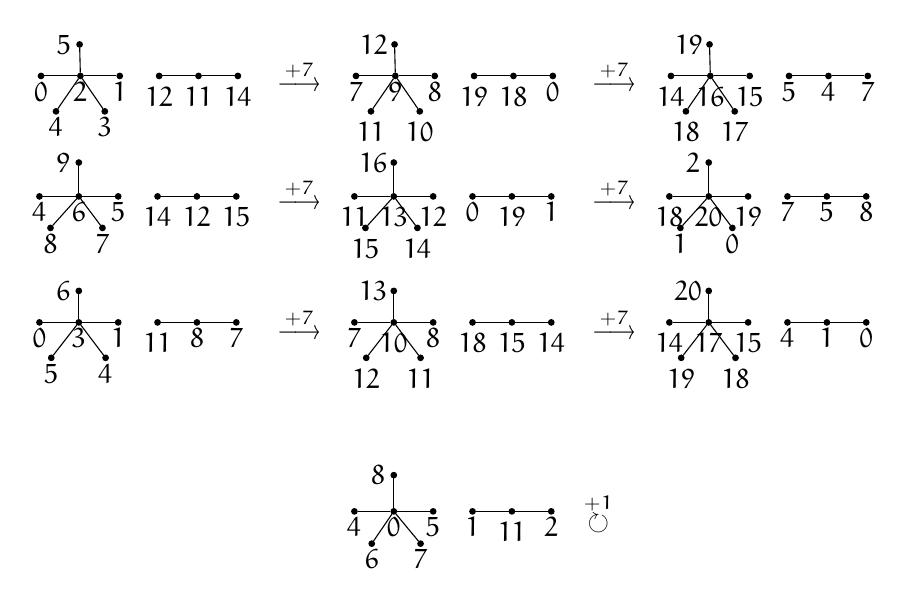
\begin{tikzpicture}[every node/.style={draw, circle, fill=black, minimum size=2pt, inner sep=0pt}]
        \node[fill=black, label=below:{\color{black}$0$}] (G1N0) at (3.72,7.33) {};
        \node[fill=black, label=below:{\color{black}$2$}] (G1N2) at (4.22,7.33) {};
        \node[fill=black, label=below:{\color{black}$1$}] (G1N1) at (4.72,7.33) {};
        \node[fill=black, label=below:{\color{black}$3$}] (G1N3) at (4.53,6.88) {};
        \node[fill=black, label=below:{\color{black}$4$}] (G1N4) at (3.91,6.88) {};
        \node[fill=black, label=left:{\color{black}$5$}] (G1N5) at (4.21,7.73) {};
        \node[fill=black, label=below:{\color{black}$12$}] (G1N12) at (5.22,7.33) {};
        \node[fill=black, label=below:{\color{black}$11$}] (G1N11) at (5.72,7.33) {};
        \node[fill=black, label=below:{\color{black}$14$}] (G1N14) at (6.22,7.33) {};
        \draw (G1N2) -- (G1N0);
        \draw (G1N2) -- (G1N1);
        \draw (G1N2) -- (G1N3);
        \draw (G1N2) -- (G1N4);
        \draw (G1N2) -- (G1N5);
        \draw (G1N12) -- (G1N11);
        \draw (G1N11) -- (G1N14);
        \node[fill=black, label=below:{\color{black}$4$}] (G2N4) at (3.70,5.80) {};
        \node[fill=black, label=below:{\color{black}$6$}] (G2N6) at (4.20,5.80) {};
        \node[fill=black, label=below:{\color{black}$5$}] (G2N5) at (4.70,5.80) {};
        \node[fill=black, label=below:{\color{black}$7$}] (G2N7) at (4.50,5.40) {};
        \node[fill=black, label=below:{\color{black}$8$}] (G2N8) at (3.84,5.40) {};
        \node[fill=black, label=left:{\color{black}$9$}] (G2N9) at (4.20,6.23) {};
        \node[fill=black, label=below:{\color{black}$14$}] (G2N14) at (5.20,5.80) {};
        \node[fill=black, label=below:{\color{black}$12$}] (G2N12) at (5.70,5.80) {};
        \node[fill=black, label=below:{\color{black}$15$}] (G2N15) at (6.20,5.80) {};
        \draw (G2N6) -- (G2N4);
        \draw (G2N6) -- (G2N5);
        \draw (G2N6) -- (G2N7);
        \draw (G2N6) -- (G2N8);
        \draw (G2N6) -- (G2N9);
        \draw (G2N14) -- (G2N12);
        \draw (G2N12) -- (G2N15);
        \node[fill=black, label=below:{\color{black}$0$}] (G3N0) at (3.70,4.20) {};
        \node[fill=black, label=below:{\color{black}$3$}] (G3N3) at (4.20,4.20) {};
        \node[fill=black, label=below:{\color{black}$1$}] (G3N1) at (4.70,4.20) {};
        \node[fill=black, label=below:{\color{black}$4$}] (G3N4) at (4.54,3.75) {};
        \node[fill=black, label=below:{\color{black}$5$}] (G3N5) at (3.85,3.75) {};
        \node[fill=black, label=left:{\color{black}$6$}] (G3N6) at (4.20,4.6) {};
        \node[fill=black, label=below:{\color{black}$11$}] (G3N11) at (5.20,4.20) {};
        \node[fill=black, label=below:{\color{black}$8$}] (G3N8) at (5.70,4.20) {};
        \node[fill=black, label=below:{\color{black}$7$}] (G3N7) at (6.20,4.20) {};
        \draw (G3N3) -- (G3N0);
        \draw (G3N3) -- (G3N1);
        \draw (G3N3) -- (G3N4);
        \draw (G3N3) -- (G3N5);
        \draw (G3N3) -- (G3N6);
        \draw (G3N11) -- (G3N8);
        \draw (G3N8) -- (G3N7);
        \begin{scope}[xshift=3cm]
            \draw[->] (3.75,7.33) -- (4.25,7.33) node[draw = none,midway, text=black, fill=white] {$\overset{+7}{\longrightarrow}$};

            \draw[->] (3.75,5.83) -- (4.25,5.83) node[draw = none,midway, text=black, fill=white] {$\overset{+7}{\longrightarrow}$};

            \draw[->] (3.75,4.18) -- (4.25,4.18) node[draw = none,midway, text=black, fill=white] {$\overset{+7}{\longrightarrow}$};
        \end{scope}

        \begin{scope}[xshift=4cm]
            
                \node[fill=black, label=below:{\color{black}$7$}] (G1N0) at (3.72,7.33) {};
                \node[fill=black, label=below:{\color{black}$9$}] (G1N2) at (4.22,7.33) {};
                \node[fill=black, label=below:{\color{black}$8$}] (G1N1) at (4.72,7.33) {};
                \node[fill=black, label=below:{\color{black}$10$}] (G1N3) at (4.53,6.88) {};
                \node[fill=black, label=below:{\color{black}$11$}] (G1N4) at (3.91,6.88) {};
                \node[fill=black, label=left:{\color{black}$12$}] (G1N5) at (4.21,7.73) {};
                \node[fill=black, label=below:{\color{black}$19$}] (G1N12) at (5.22,7.33) {};
                \node[fill=black, label=below:{\color{black}$18$}] (G1N11) at (5.72,7.33) {};
                \node[fill=black, label=below:{\color{black}$0$}] (G1N14) at (6.22,7.33) {};
                \draw (G1N2) -- (G1N0);
                \draw (G1N2) -- (G1N1);
                \draw (G1N2) -- (G1N3);
                \draw (G1N2) -- (G1N4);
                \draw (G1N2) -- (G1N5);
                \draw (G1N12) -- (G1N11);
                \draw (G1N11) -- (G1N14);
                \node[fill=black, label=below:{\color{black}$11$}] (G2N4) at (3.70,5.80) {};
                \node[fill=black, label=below:{\color{black}$13$}] (G2N6) at (4.20,5.80) {};
                \node[fill=black, label=below:{\color{black}$12$}] (G2N5) at (4.70,5.80) {};
                \node[fill=black, label=below:{\color{black}$14$}] (G2N7) at (4.50,5.40) {};
                \node[fill=black, label=below:{\color{black}$15$}] (G2N8) at (3.84,5.40) {};
                \node[fill=black, label=left:{\color{black}$16$}] (G2N9) at (4.20,6.23) {};
                \node[fill=black, label=below:{\color{black}$0$}] (G2N14) at (5.20,5.80) {};
                \node[fill=black, label=below:{\color{black}$19$}] (G2N12) at (5.70,5.80) {};
                \node[fill=black, label=below:{\color{black}$1$}] (G2N15) at (6.20,5.80) {};
                \draw (G2N6) -- (G2N4);
                \draw (G2N6) -- (G2N5);
                \draw (G2N6) -- (G2N7);
                \draw (G2N6) -- (G2N8);
                \draw (G2N6) -- (G2N9);
                \draw (G2N14) -- (G2N12);
                \draw (G2N12) -- (G2N15);
                \node[fill=black, label=below:{\color{black}$7$}] (G3N0) at (3.70,4.20) {};
                \node[fill=black, label=below:{\color{black}$10$}] (G3N3) at (4.20,4.20) {};
                \node[fill=black, label=below:{\color{black}$8$}] (G3N1) at (4.70,4.20) {};
                \node[fill=black, label=below:{\color{black}$11$}] (G3N4) at (4.54,3.75) {};
                \node[fill=black, label=below:{\color{black}$12$}] (G3N5) at (3.85,3.75) {};
                \node[fill=black, label=left:{\color{black}$13$}] (G3N6) at (4.20,4.6) {};
                \node[fill=black, label=below:{\color{black}$18$}] (G3N11) at (5.20,4.20) {};
                \node[fill=black, label=below:{\color{black}$15$}] (G3N8) at (5.70,4.20) {};
                \node[fill=black, label=below:{\color{black}$14$}] (G3N7) at (6.20,4.20) {};
                \draw (G3N3) -- (G3N0);
                \draw (G3N3) -- (G3N1);
                \draw (G3N3) -- (G3N4);
                \draw (G3N3) -- (G3N5);
                \draw (G3N3) -- (G3N6);
                \draw (G3N11) -- (G3N8);
                \draw (G3N8) -- (G3N7);
                \node[fill=black, label=below:{\color{black}$4$}] (G4N4) at (3.70,1.80) {};
        \node[fill=black, label=below:{\color{black}$0$}] (G4N0) at (4.20,1.80) {};
        \node[fill=black, label=below:{\color{black}$5$}] (G4N5) at (4.70,1.80) {};
        \node[fill=black, label=below:{\color{black}$6$}] (G4N6) at (3.92,1.39) {};
        \node[fill=black, label=below:{\color{black}$7$}] (G4N7) at (4.54,1.39) {};
        \node[fill=black, label=left:{\color{black}$8$}] (G4N8) at (4.20,2.26) {};
        \node[fill=black, label=below:{\color{black}$1$}] (G4N1) at (5.20,1.80) {};
        \node[fill=black, label=below:{\color{black}$11$}] (G4N11) at (5.70,1.80) {};
        \node[fill=black, label=below:{\color{black}$2$}] (G4N2) at (6.20,1.80) {};
        \draw (G4N0) -- (G4N4);
        \draw (G4N0) -- (G4N5);
        \draw (G4N0) -- (G4N6);
        \draw (G4N0) -- (G4N7);
        \draw (G4N0) -- (G4N8);
        \draw (G4N1) -- (G4N11);
        \draw (G4N11) -- (G4N2);
        
            \draw[->] (6.8,1.78) -- (6.8,1.78) node[draw = none,midway, text=black, fill=white] {$\overset{+1}{\circlearrowright}$};

        \end{scope}
        \begin{scope}[xshift=7cm]
            \draw[->] (3.75,7.33) -- (4.25,7.33) node[draw = none,midway, text=black, fill=white] {$\overset{+7}{\longrightarrow}$};

            \draw[->] (3.75,5.83) -- (4.25,5.83) node[draw = none,midway, text=black, fill=white] {$\overset{+7}{\longrightarrow}$};

            \draw[->] (3.75,4.18) -- (4.25,4.18) node[draw = none,midway, text=black, fill=white] {$\overset{+7}{\longrightarrow}$};
        \end{scope}
        \begin{scope}[xshift = 8cm]

                \node[fill=black, label=below:{\color{black}$14$}] (G1N0) at (3.72,7.33) {};
                \node[fill=black, label=below:{\color{black}$16$}] (G1N2) at (4.22,7.33) {};
                \node[fill=black, label=below:{\color{black}$15$}] (G1N1) at (4.72,7.33) {};
                \node[fill=black, label=below:{\color{black}$17$}] (G1N3) at (4.53,6.88) {};
                \node[fill=black, label=below:{\color{black}$18$}] (G1N4) at (3.91,6.88) {};
                \node[fill=black, label=left:{\color{black}$19$}] (G1N5) at (4.21,7.73) {};
                \node[fill=black, label=below:{\color{black}$5$}] (G1N12) at (5.22,7.33) {};
                \node[fill=black, label=below:{\color{black}$4$}] (G1N11) at (5.72,7.33) {};
                \node[fill=black, label=below:{\color{black}$7$}] (G1N14) at (6.22,7.33) {};
                \draw (G1N2) -- (G1N0);
                \draw (G1N2) -- (G1N1);
                \draw (G1N2) -- (G1N3);
                \draw (G1N2) -- (G1N4);
                \draw (G1N2) -- (G1N5);
                \draw (G1N12) -- (G1N11);
                \draw (G1N11) -- (G1N14);
                \node[fill=black, label=below:{\color{black}$18$}] (G2N4) at (3.70,5.80) {};
                \node[fill=black, label=below:{\color{black}$20$}] (G2N6) at (4.20,5.80) {};
                \node[fill=black, label=below:{\color{black}$19$}] (G2N5) at (4.70,5.80) {};
                \node[fill=black, label=below:{\color{black}$0$}] (G2N7) at (4.50,5.40) {};
                \node[fill=black, label=below:{\color{black}$1$}] (G2N8) at (3.84,5.40) {};
                \node[fill=black, label=left:{\color{black}$2$}] (G2N9) at (4.20,6.23) {};
                \node[fill=black, label=below:{\color{black}$7$}] (G2N14) at (5.20,5.80) {};
                \node[fill=black, label=below:{\color{black}$5$}] (G2N12) at (5.70,5.80) {};
                \node[fill=black, label=below:{\color{black}$8$}] (G2N15) at (6.20,5.80) {};
                \draw (G2N6) -- (G2N4);
                \draw (G2N6) -- (G2N5);
                \draw (G2N6) -- (G2N7);
                \draw (G2N6) -- (G2N8);
                \draw (G2N6) -- (G2N9);
                \draw (G2N14) -- (G2N12);
                \draw (G2N12) -- (G2N15);
                \node[fill=black, label=below:{\color{black}$14$}] (G3N0) at (3.70,4.20) {};
                \node[fill=black, label=below:{\color{black}$17$}] (G3N3) at (4.20,4.20) {};
                \node[fill=black, label=below:{\color{black}$15$}] (G3N1) at (4.70,4.20) {};
                \node[fill=black, label=below:{\color{black}$18$}] (G3N4) at (4.54,3.75) {};
                \node[fill=black, label=below:{\color{black}$19$}] (G3N5) at (3.85,3.75) {};
                \node[fill=black, label=left:{\color{black}$20$}] (G3N6) at (4.20,4.6) {};
                \node[fill=black, label=below:{\color{black}$4$}] (G3N11) at (5.20,4.20) {};
                \node[fill=black, label=below:{\color{black}$1$}] (G3N8) at (5.70,4.20) {};
                \node[fill=black, label=below:{\color{black}$0$}] (G3N7) at (6.20,4.20) {};
                \draw (G3N3) -- (G3N0);
                \draw (G3N3) -- (G3N1);
                \draw (G3N3) -- (G3N4);
                \draw (G3N3) -- (G3N5);
                \draw (G3N3) -- (G3N6);
                \draw (G3N11) -- (G3N8);
                \draw (G3N8) -- (G3N7);
                
        
        \end{scope}
        \end{tikzpicture}
\end{frame}

\section{$K_{1,7}\sqcup P_{2}$}

\begin{frame}{$K_{1,7}\sqcup P_{2}$}
\textbf{We were unable to find (1-2-3) and 1-rotational (1-2-3) labelings for exactly one graph (by hand and using a constraint programming algorithm). So we took a completely different approach for this exceptional graph $K_{1,7}\sqcup P_{2}$.}\newline
\begin{itemize}
    \item In 1974, Pauline Cain proved that there exists an $K_{1,7}-$design of order $21$. She provided a construction, which is based on partitioning $K_{21}$ into three joined copies of $K_{7}$. 
    
    \pause
    
    \item By 'peeling' an edge off each $7$-edge star in this decomposition, we seperated the decomposition into resulting in 30 $6$-edge stars and 30 single edge paths. We paired the paths with a vertex disjoint $6$-edge star, and these 30 unions resulted in a $K_{1,7}\sqcup P_{2}$-design of order $21$.
    
    \pause

    \item We obtained the $K_{1,7}\sqcup P_{2}$-design of order $21$ by adding the $\infty$ node and it's new edges to this $K_{1,7}\sqcup P_{2}$-design of order $21$ and changing some pairings.
    
\end{itemize}

\end{frame}

\begin{frame}{$K_{1,7}\sqcup P_{2}$-decomposition of $K_{7:7}$ and $K_{8:7}$}

\textbf{Why did we do this?}\newline

\begin{itemize}

    \item We begin this case by constructing $K_{n}$ for $n \equiv 7 \textrm{ or } 8 \pmod{14}$ and $n\geq 21$ using \textit{joined} copies of $K_{22}$, $K_{21}$, and $K_{14}$. The \textit{join} of two graphs $G_{1}$ and $G_{2}$ is the graph obtained by adding an edge $\{g_1,g_2\}$ for every vertex $g_1 \in V(G_{1})$ and every vertex of $g_2 \in V(G_{2})$.

    \item Let $t$ be a positive integer and join $t-1$ copies of $K_{14}$ with each other and a lone copy of $K_{21}$. The resulting graph is $K_{14(t-1)+21} \cong K_{14t+7}$. So we can think of $K_{14t+7}$ as $K_{t}$ whose $t$ ``vertices'' consist of $t-1$ copies of $K_{14}$ and $1$ copy of $K_{21}$ and whose edges are the join between them. From now on, we will refer to these ``vertices'' as nodes. Similarly, $K_{14t+8}$ can be constructed as $K_{t}$ whose nodes are $t-1$ copies of $K_{14}$ and $1$ copy of $K_{22}$ and whose edges are the join between them.

\end{itemize}

We show a figure to illustrate this construction on the next slide.

\end{frame}

\begin{frame}{Special Construction for $K_{14t+7}$ and $K_{14t+8}$}
%%%%%%%%%%%%%%%%%%%%%%%%%%%%%%%%%%%%%%%%%%%%%%%%%%%%%%%%%%%%%%%%%%%%%%%%%%%%%%%%%%%%%%%%%%%%%%%%%%%%%%%%%%%%%%%%%%%%%%%%%%%
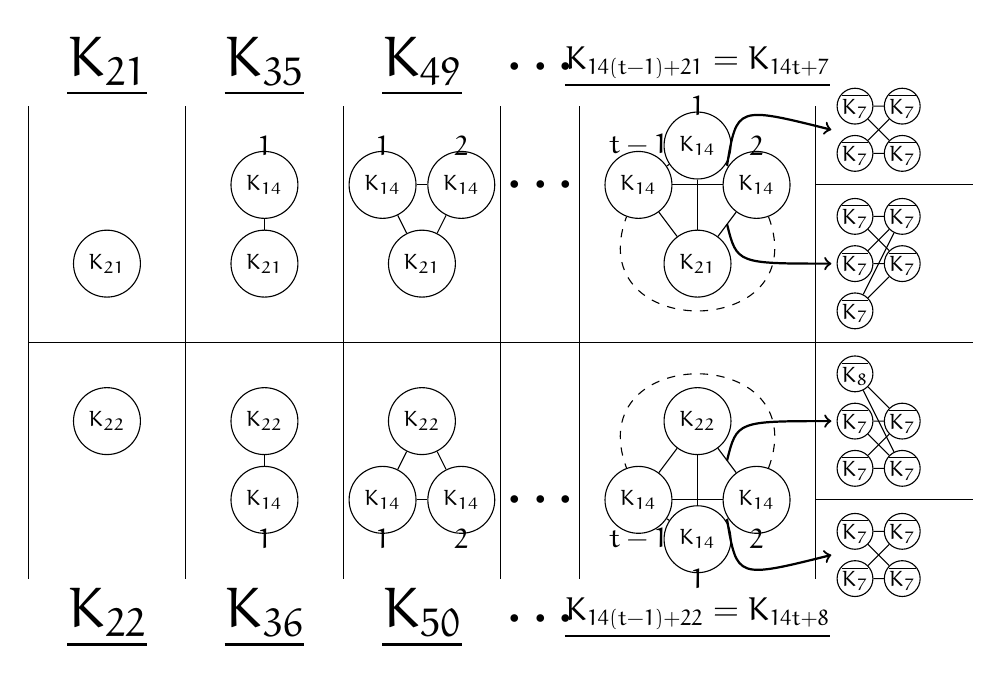
\begin{tikzpicture}
    % Original Top Part
    % K_21 (HEADER)
    \node at (0,4.5) {\huge $\underline{K_{21}}$};
    \node[draw, circle] (K21) at (0, 2) {\footnotesize $K_{21}$};

    % Solid dividers
    \draw[solid] (-1,4) --(-1,-2);
    \draw[solid] (1,4) -- (1,-2);
    \draw[solid] (3,4) -- (3,-2);
    \draw[solid] (5,4) -- (5,-2);
    \draw[solid] (6,4) -- (6,-2);
    \draw[solid] (9,4) -- (9,-2);

    \draw[solid] (-1,1) -- (11,1);
    \draw[solid] (9,3) -- (11,3);
    \draw[solid] (9,-1) -- (11,-1);

    % K_35
    \begin{scope}[shift={(2,2)}]
        \node at (0,2.5) {\huge $\underline{K_{35}}$};
        \node[draw, circle] (K21) at (0, 0) {\footnotesize $K_{21}$};
        \node at (0, 1.5) {$1$};
        \node[draw, circle] (K141) at (0, 1) {\footnotesize $K_{14}$};
        \draw (K21)--(K141);
    \end{scope}

    % K_49
    \begin{scope}[shift={(4,2)}]
        \node at (0,2.5) {\huge $\underline{K_{49}}$};
        \node[draw, circle] (K21) at (0, 0) {\footnotesize $K_{21}$};

        \node at (-0.5, 1.5) {$1$};
        \node[draw, circle] (K141) at (-0.5, 1) {\footnotesize $K_{14}$};

        \node at (0.5, 1.5) {$2$};
        \node[draw, circle] (K142) at (0.5, 1) {\footnotesize $K_{14}$};

        \draw (K21)--(K141);
        \draw (K21)--(K142);
        \draw (K141)--(K142);
    \end{scope}  

    % Big \hdots
    \node at (5.5,4.5) {\huge $\hdots$};
    \node at (5.5,3) {\huge $\hdots$};

    % K_14t+7
    \begin{scope}[shift={(7.5,2)}]
        \node at (0,2.5) {\large $\underline{K_{14(t-1)+21}=K_{14t+7}}$};
        \node[draw, circle] (K21) at (0, 0) {\footnotesize $K_{21}$};

        \node at (-0.75, 1.5) {$t-1$};
        \node[draw, circle] (K141) at (-0.75, 1) {\footnotesize $K_{14}$};

        \node at (0, 2) {$1$};
        \node[draw, circle] (K142) at (0, 1.5) {\footnotesize $K_{14}$};

        \node at (0.75, 1.5) {$2$};
        \node[draw, circle] (K143) at (0.75, 1) {\footnotesize $K_{14}$};

        \draw (K21)--(K141);
        \draw (K21)--(K142);
        \draw (K21)--(K143);
        \draw (K141)--(K142);
        \draw (K141)--(K143);
        \draw (K142)--(K143);

        % Large arcing dotted edge from K143 to K141 orbiting K21
        \draw[dashed] (K143) .. controls (1.5, -1) and (-1.5, -1) .. (K141);
    \end{scope}
    %K_14,14
    \begin{scope}[shift={(9.5,4)}]
        \node[draw, circle, minimum size=11pt, inner sep=0pt] (AK71) at (0, 0) {\footnotesize $\overline{K_{7}}$};
        \node[draw, circle, minimum size=11pt, inner sep=0pt] (AK72) at (0, -0.6) {\footnotesize $\overline{K_{7}}$};

        \node[draw, circle, minimum size=11pt, inner sep=0pt] (BK71) at (0.6, 0) {\footnotesize $\overline{K_{7}}$};
        \node[draw, circle, minimum size=11pt, inner sep=0pt] (BK72) at (0.6, -0.6) {\footnotesize $\overline{K_{7}}$};

        \draw (AK71)--(BK71)--(AK72);
        \draw (AK72)--(BK72)--(AK71);

    \end{scope}
    %% ARROW 1
        % Calculate the midpoint of K142-K143
        \path (K142) -- (K143) coordinate[midway] (M1);

        % Calculate the midpoint of AK71-AK72
        \path (AK71) -- (AK72) coordinate[midway] (M2);

        \path (M2)++(-0.3,0) coordinate (M2);
    
        % Draw a bent solid arrow through (7.75,4)
        \draw[->, thick] (M1) .. controls (8,4) .. (M2);

    \begin{scope}[shift={(9.5,2.6)}]
        \node[draw, circle, minimum size=11pt, inner sep=0pt] (AK71) at (0, 0) {\footnotesize $\overline{K_{7}}$};
        \node[draw, circle, minimum size=11pt, inner sep=0pt] (AK72) at (0, -0.6) {\footnotesize $\overline{K_{7}}$};
        \node[draw, circle, minimum size=11pt, inner sep=0pt] (AK73) at (0, -1.2) {\footnotesize $\overline{K_{7}}$};


        \node[draw, circle, minimum size=11pt, inner sep=0pt] (BK71) at (0.6, 0) {\footnotesize $\overline{K_{7}}$};
        \node[draw, circle, minimum size=11pt, inner sep=0pt] (BK72) at (0.6, -0.6) {\footnotesize $\overline{K_{7}}$};

        \draw (AK71)--(BK71)--(AK72);
        \draw (AK72)--(BK72)--(AK71);
        \draw (BK71)--(AK73)--(BK72);

    \end{scope}
    %% ARROW 2

        % Calculate the midpoint of K142-K143
    \path (K21) -- (K143) coordinate[midway] (M1);

    % Shift the endpoint left by (-0.3,0)
    \path (AK72) ++(-0.3,0) coordinate (M2);

    % Draw a bent solid arrow through (7.75,4)
    \draw[->, thick] (M1) .. controls (8,2) .. (M2);


    %% mirrored

    
    %----------------------------------------------------------------------------------------------------------------------
    
    

    \begin{scope}[shift={(9.5,0.6)}]
        \node[draw, circle, minimum size=11pt, inner sep=0pt] (AK81) at (0, 0) {\footnotesize $\overline{K_{8}}$};
        \node[draw, circle, minimum size=11pt, inner sep=0pt] (AK72) at (0, -0.6) {\footnotesize $\overline{K_{7}}$};
        \node[draw, circle, minimum size=11pt, inner sep=0pt] (AK73) at (0, -1.2) {\footnotesize $\overline{K_{7}}$};


        \node[draw, circle, minimum size=11pt, inner sep=0pt] (BK71) at (0.6, -0.6) {\footnotesize $\overline{K_{7}}$};
        \node[draw, circle, minimum size=11pt, inner sep=0pt] (BK72) at (0.6, -1.2) {\footnotesize $\overline{K_{7}}$};

        \draw (AK81)--(BK71)--(AK72);
        \draw (AK72)--(BK72)--(AK81);
        \draw (BK71)--(AK73)--(BK72);

    \end{scope}

    \begin{scope}[shift={(9.5,-1.4)}]
        \node[draw, circle, minimum size=11pt, inner sep=0pt] (AK71) at (0, 0) {\footnotesize $\overline{K_{7}}$};
        \node[draw, circle, minimum size=11pt, inner sep=0pt] (AK72) at (0, -0.6) {\footnotesize $\overline{K_{7}}$};

        \node[draw, circle, minimum size=11pt, inner sep=0pt] (BK71) at (0.6, 0) {\footnotesize $\overline{K_{7}}$};
        \node[draw, circle, minimum size=11pt, inner sep=0pt] (BK72) at (0.6, -0.6) {\footnotesize $\overline{K_{7}}$};

        \draw (AK71)--(BK71)--(AK72);
        \draw (AK72)--(BK72)--(AK71);

    \end{scope}


    % REFLECTED SECTION BELOW Y = 0
    % K_22 (Reflected)
    \node at (0,-2.5) {\huge $\underline{K_{22}}$};
    \node[draw, circle] (K21) at (0, 0) {\footnotesize $K_{22}$};

    % K_35 (Reflected)
    \begin{scope}[shift={(2,0)}]
        \node at (0,-2.5) {\huge $\underline{K_{36}}$};
        \node[draw, circle] (K21) at (0, 0) {\footnotesize $K_{22}$};
        \node at (0, -1.5) {$1$};
        \node[draw, circle] (K141) at (0, -1) {\footnotesize $K_{14}$};
        \draw (K21)--(K141);
    \end{scope}

    % K_49 (Reflected)
    \begin{scope}[shift={(4,0)}]
        \node at (0,-2.5) {\huge $\underline{K_{50}}$};
        \node[draw, circle] (K21) at (0, 0) {\footnotesize $K_{22}$};

        \node at (-0.5, -1.5) {$1$};
        \node[draw, circle] (K141) at (-0.5, -1) {\footnotesize $K_{14}$};

        \node at (0.5, -1.5) {$2$};
        \node[draw, circle] (K142) at (0.5, -1) {\footnotesize $K_{14}$};

        \draw (K21)--(K141);
        \draw (K21)--(K142);
        \draw (K141)--(K142);
    \end{scope}  

    % Big \hdots (Reflected)
    \node at (5.5,-2.5) {\huge $\hdots$};
    \node at (5.5,-1) {\huge $\hdots$};

    % K_14t+7 (Reflected)
    \begin{scope}[shift={(7.5,0)}]
        \node at (0,-2.5) {\large $\underline{K_{14(t-1)+22}=K_{14t+8}}$};
        \node[draw, circle] (K21) at (0, 0) {\footnotesize $K_{22}$};

        \node at (-0.75, -1.5) {$t-1$};
        \node[draw, circle] (K141) at (-0.75, -1) {\footnotesize $K_{14}$};

        \node at (0, -2) {$1$};
        \node[draw, circle] (K142) at (0, -1.5) {\footnotesize $K_{14}$};

        \node at (0.75, -1.5) {$2$};
        \node[draw, circle] (K143) at (0.75, -1) {\footnotesize $K_{14}$};

        \draw (K21)--(K141);
        \draw (K21)--(K142);
        \draw (K21)--(K143);
        \draw (K141)--(K142);
        \draw (K141)--(K143);
        \draw (K142)--(K143);

        % Large arcing dotted edge from K143 to K141 orbiting K21 (Reflected)
        \draw[dashed] (K143) .. controls (1.5, 1) and (-1.5, 1) .. (K141);
    \end{scope}

    %% MIRRORED ARROW 1
    % Calculate the midpoint of K142-K143
    \path (K142) -- (K143) coordinate[midway] (M1);

    % Calculate the midpoint of AK71-AK72
    \path (AK71) -- (AK72) coordinate[midway] (M2);

    \path (M2)++(-0.3,0) coordinate (M2);

    % Draw a bent solid arrow through (7.75,4)
    \draw[->, thick] (M1) .. controls (8,-2) .. (M2);

    %% MIRRORED ARROW 2

    \path (K21) -- (K143) coordinate[midway] (M1);

    % Shift the endpoint left by (-0.3,0)
    \path (AK81) ++(-0.3,-0.6) coordinate (M2);

    % Draw a bent solid arrow through (7.75,4)
    \draw[->, thick] (M1) .. controls (8,0) .. (M2);

\end{tikzpicture}

%%%%%%%%%%%%%%%%%%%%%%%%%%%%%%%%%%%%%%%%%%%%%%%%%%%%%%%%%%%%%%%%%%%%%%%%%%%%%%%%%%%%%%%%%%%%%%%%%%%%%%%%%%%%%%%%%%%%%%%%%%%

\end{frame}

\begin{frame}{Building the decompositions piece-by-piece}

    \begin{itemize}
        \item We show that $K_{1,7}\sqcup P_{2}$ decomposes $K_{n}$ for $n\equiv7 \textrm{ or }8\pmod{14}$ by proving $K_{22},K_{21},K_{14},K_{22,14},K_{21,14},\text{ and }K_{14,14}$ are each $K_{1,7}\sqcup P_{2}$-decomposable. Notice that these 6 graphs make up the nodes and edges of the $K_{t}$ representations of $K_{14t+7}$ and $K_{14t+8}$ stated in the constructions above.
        \pause
        \item We have already proven that $K_{14}$, $K_{21}$, and $K_{22}$ are $K_{1,7}\sqcup P_{2}$-decomposable. So all we need to do is prove $K_{22,14},K_{21,14},\text{ and }K_{14,14}$ are also $K_{1,7}\sqcup P_{2}$-decomposable.
        \pause

    \end{itemize}
    \begin{center}
    \textbf{We do so in style. See the figure below.}
    \end{center}
\begin{figure}
\begin{center}
    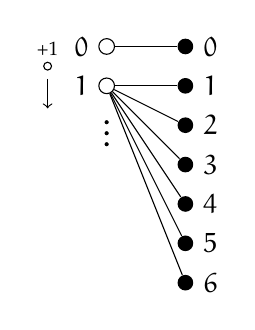
\begin{tikzpicture}[scale=0.5]
        %white
        \node[fill=white,draw =black, circle, inner sep=2pt, label=left:{\textcolor{black}{$0$}}] (w0) at (0,0) {};
        \node[fill=white,draw = black, circle, inner sep=2pt, label=left:{\textcolor{black}{$1$}}] (w1) at (0,-1) {};
        \node at (0,-2) {\large $\vdots$};

        \node[draw=black, fill=white, circle, inner sep=1pt] (circ) at (-1.5,-0.5) {};
        \node at ([yshift=9pt] circ.north) {\scriptsize +1};
        \draw[->] ([yshift=-6pt] circ.south) -- ++(0, -0.75);
        %black nodes
        \node[fill=black, circle, inner sep=2pt, label=right:{\textcolor{black}{$0$}}] (b0) at (2,0) {};
        \node[fill=black, circle, inner sep=2pt, label=right:{\textcolor{black}{$1$}}] (b1) at (2,-1) {};
        \node[fill=black, circle, inner sep=2pt, label=right:{\textcolor{black}{$2$}}] (b2) at (2,-2) {};
        \node[fill=black, circle, inner sep=2pt, label=right:{\textcolor{black}{$3$}}] (b3) at (2,-3) {};
        \node[fill=black, circle, inner sep=2pt, label=right:{\textcolor{black}{$4$}}] (b4) at (2,-4) {};
        \node[fill=black, circle, inner sep=2pt, label=right:{\textcolor{black}{$5$}}] (b5) at (2,-5) {};
        \node[fill=black, circle, inner sep=2pt, label=right:{\textcolor{black}{$6$}}] (b6) at (2,-6) {};
        \node at (0,-2) {\large $\vdots$};

        \draw[draw=black, shorten >=0pt, shorten <=0pt] (w0) -- (b0);
        \draw[draw=black, shorten >=0pt, shorten <=0pt] (w1) -- (b1);
        \draw[draw=black, shorten >=0pt, shorten <=0pt] (w1) -- (b2);
        \draw[draw=black, shorten >=0pt, shorten <=0pt] (w1) -- (b3);
        \draw[draw=black, shorten >=0pt, shorten <=0pt] (w1) -- (b4);
        \draw[draw=black, shorten >=0pt, shorten <=0pt] (w1) -- (b5);
        \draw[draw=black, shorten >=0pt, shorten <=0pt] (w1) -- (b6);
    \end{tikzpicture}
\end{center}
\caption{A generating presentation of the $K_{1,7}\sqcup P_{2}$-decomposition of $K_{n,7}$ for $n\geq 2$}
\end{figure}
\end{frame}

\begin{frame}{Finally!}
We get these theorems as a result of this fun left generated labeling:

\begin{theorem}
$K_{1,7}\sqcup P_{2}$-decomposes $K_{n,7}$ for all $n\geq 2$.
\end{theorem}

\begin{theorem}
$K_{1,7}\sqcup P_{2}$ decomposes $K_{22,14}$, $K_{21,14},\text{ and }K_{14,14}$.
\end{theorem}

\begin{proof}
    Notice $K_{14,14}$ can be expressed as the edge-disjoint union of four copies of $K_{7,7}$, $K_{21,14}$ can be expressed as the edge-disjoint union of six copies of $K_{7,7}$, and $K_{22,14}$ can be expressed as the edge-disjoint union of two copies of $K_{8,7}$ and four copies of $K_{7,7}$. Therefore, $K_{1,7}\sqcup P_{2}$ decomposes them all. This is visualized in a previous figure.
\end{proof}
So finally...
\begin{theorem}
There exists a seven edge forest design of order $n$ if and only if $n\equiv 0,1,7\text{ or }8\Mod{14}$.
\end{theorem}
\end{frame}

\begin{frame}{A bonus result!}
From this one-sided cyclic permutation idea, we can generalize this bipartite idea to a special subset of forest graphs called \textit{Galaxy} graphs whose connected components are all star graphs.

\begin{theorem}
Let $C=\{G_{1},\hdots, G_{n}\}$ be a set of vertex disjoint star graphs, $x_{i}=k$ if $G_{i}\cong K_{1,k}$, and $m=\sum_{i=1}^{n} x_{i}$. The Galaxy graph $\GG=\bigsqcup_{G\in C} G$ decomposes $K_{N,m}$ for all $N>n$. 
\end{theorem}
\begin{proof}
This works the same way the $K_{1,7}\sqcup P_{2}$-labeling works. Simply color the centers of $G_{1},\hdots,G_{n}$ and label them $0,\hdots,n-1$, respectively. Now simply develop the white vertices by $1$ modulo $N$ and you get the decomposition.
\end{proof}
Naturally what follows is that such a Galaxy $\GG$ also decomposes $K_{N,M}$ where $N\geq n$ and $M$ is a multiple of $m$, and we can also extend this to $\overline{K_{N}}\lor (\overline{K_{M_{1}}}\sqcup \cdots \sqcup \overline{K_{M_{c}}})$ where all $M_{i}$'s are mutliples of $M$... and so on.
\end{frame}

\begin{frame}{Thank you!}

\begin{center}
    \textbf{Questions? -- Thank you all for coming!}
\end{center}

    \end{frame}

\end{document}
